\documentclass[12pt,reqno]{amsart}
\usepackage[pdfborder={0 0 0.5 [3 2]}, plainpages=false]{hyperref}%
\usepackage[left=1in,right=1in,top=1in,bottom=1in]{geometry}%
\usepackage[citation-order]{amsrefs}%
\usepackage{amsmath}
\usepackage{enumerate}
\usepackage{amssymb}                
\usepackage{amsfonts}
\usepackage{amsthm}
\usepackage{bbm}
\usepackage[table,xcdraw]{xcolor}
\usepackage{float}
\usepackage{mathtools}
\usepackage{cool}
\usepackage{graphicx,epsfig}

\usepackage[capitalize,nameinlink]{cleveref}
% Per SIAM Style Manual, "section" should be lowercase
\crefname{section}{section}{sections}
\crefname{subsection}{subsection}{subsections}
\Crefname{section}{Section}{Sections}
\Crefname{subsection}{Subsection}{Subsections}

% Per SIAM Style Manual, "Figure" should be spelled out in references
\Crefname{figure}{Figure}{Figures}

% Per SIAM Style Manual, don't say equation in front on an equation.
\crefformat{equation}{\textup{#2(#1)#3}}
\crefrangeformat{equation}{\textup{#3(#1)#4--#5(#2)#6}}
\crefmultiformat{equation}{\textup{#2(#1)#3}}{ and \textup{#2(#1)#3}}
{, \textup{#2(#1)#3}}{, and \textup{#2(#1)#3}}
\crefrangemultiformat{equation}{\textup{#3(#1)#4--#5(#2)#6}}%
{ and \textup{#3(#1)#4--#5(#2)#6}}{, \textup{#3(#1)#4--#5(#2)#6}}{, and \textup{#3(#1)#4--#5(#2)#6}}

% But spell it out at the beginning of a sentence.
\Crefformat{equation}{#2Equation~\textup{(#1)}#3}
\Crefrangeformat{equation}{Equations~\textup{#3(#1)#4--#5(#2)#6}}
\Crefmultiformat{equation}{Equations~\textup{#2(#1)#3}}{ and \textup{#2(#1)#3}}
{, \textup{#2(#1)#3}}{, and \textup{#2(#1)#3}}
\Crefrangemultiformat{equation}{Equations~\textup{#3(#1)#4--#5(#2)#6}}%
{ and \textup{#3(#1)#4--#5(#2)#6}}{, \textup{#3(#1)#4--#5(#2)#6}}{, and \textup{#3(#1)#4--#5(#2)#6}}

% Make number non-italic in any environment.
\crefdefaultlabelformat{#2\textup{#1}#3}

\def\noi{\noindent}
\def\T{{\mathbb T}}
\def\R{{\mathbb R}}
\def\N{{\mathbb N}}
\def\C{{\mathbb C}}
\def\Z{{\mathbb Z}}
\def\P{{\mathbb P}}
\def\E{{\mathbb E}}
\def\Q{\mathbb{Q}}
\def\ind{{\mathbb I}}
\def\id{{\mathcal I}}
\def\per{\textrm{per}}
\def\calL{\mathcal{L}}
\def\calI{\mathcal{I}}

\newcommand{\uvec}{\mathbf{u}}
\newcommand{\vvec}{\mathbf{v}}
\newcommand{\wvec}{\mathbf{w}}
\newcommand{\zvec}{\mathbf{z}}

\DeclareMathOperator{\spn}{span}
\DeclareMathOperator{\ran}{range}

\graphicspath{ {images/} }

\newtheorem{lemma}{Lemma}
\newtheorem{theorem}{Theorem}
\newtheorem{corollary}{Corollary}
\newtheorem{definition}{Definition}
\newtheorem{proposition}{Proposition}
\newtheorem{hypothesis}{Hypothesis}
\newtheorem{remark}{Remark}

\newcommand{\revised}[1]{ \textcolor{red}{#1} }
\newcommand{\revisedd}[2]{ \textcolor{blue}{#1} }

\begin{document}

\title{Multi-breathers in the discrete sine-Gordon equation}

\author{Ross Parker}
\address{Department of Mathematics, Southern Methodist University, 
Dallas, TX 75275, USA}
\email{rhparker@smu.edu}

\author{P.\,G. Kevrekidis} 
\address{Department of Mathematics and Statistics, University of Massachusetts, Amherst MA 01003, USA}
\email{kevrekid@math.umass.edu}

\author{Alejandro Aceves}
\address{Department of Mathematics, Southern Methodist University, 
Dallas, TX 75275, USA}
\email{aaceves@smu.edu}

\begin{abstract}
	We consider the existence and spectral stability of multi-site breathers in the discrete Klein-Gordon equation.
\end{abstract}

\maketitle

\section{Introduction}

\section{Mathematical background}\label{sec:bg}

We will consider the discrete Klein-Gordon equation with on-site nonlinearity $f(u)$
\begin{equation}\label{eq:DKG}
\ddot{u}_n = d (\Delta_2 u)_n - f(u_n),
\end{equation}
on the integer lattice $\Z$, where $u_n(t) \in \R$, $(\Delta_2 u)_n = u_{n+1} - 2 u_n + u_{n-1}$ is the discrete second difference operator, and $f(u) = P'(u)$ for a smooth potential function $P(u)$. We make the following assumptions on the nonlinearity $f$. 
\begin{enumerate}[(i)]
	\item $f(u)$ is an odd function with $f(0) = 0$ and $f'(0) > 0$.
	\item There is a pair of nonzero equilibria $\pm u^*$ with $f(\pm u^*) = 0$ and $f'(\pm u^*) < 0$.
	\item There are no other equilibria in the interval $[-u^*, u^*]$.
\end{enumerate}
Common nonlinearities $f(u) = \sin u$, which is the discrete sine-Gordon equation, and $f(u) = u - u^3$, which is the discrete $\phi^4$ model. Equation \cref{eq:DKG} is Hamiltonian \cite{KevrekidisWeinstein2000}, with energy given by
\begin{equation}\label{eq:H}
	\mathcal{H}(u) = \sum_{n=-\infty}^\infty 
	\left( \frac{1}{2} (\dot{u}_n)^2 + \frac{d}{2} (u_{n+1} - u_n)^2 + P(u_n) \right).
\end{equation}
We are interested in breather solutions to \cref{eq:DKG}, which are periodic in time and spatially localized on the lattice. Specifically, a breather solution $\uvec$ with fundamental period $T>0$ is a solution $\uvec \in \ell^2(\Z, H^2_\per[0,T])$, where $H^2_\per[0,T]$ is the Hilbert-Sobolev space of periodic, real-valued functions on $[0,T]$. The components of $\uvec$ are denoted $u_n$, for $n \in \Z$.

To study spectral stability of a breather solution $\uvec$, we linearize equation \cref{eq:DKG} by substituting the perturbation ansatz $u_n + \epsilon v_n$ into \cref{eq:DKG} and keeping terms of order $\epsilon$ to obtain
\begin{equation}\label{eq:DKGlinear}
\ddot{v}_n = d (\Delta_2 v)_n - f'(u_n)v_n.
\end{equation}
Since $\uvec$ has period $T$, it follows from Floquet theory that spectral stability depends on the Floquet multipliers, which are the eigenvalues of the monodromy operator $\mathcal{M}$. If $\mu$ is a Floquet multiplier, then the corresponding Floquet exponent $\lambda$ (which is not unique) is related to $\mu$ by $\mu = e^{\lambda T}$. It follows (see, for example, \cite[Lemma 2.1.29]{Kapitula2013}) that for every Floquet multiplier $\mu$, there is a corresponding solution $v_n(t) = e^{\lambda t} w_n(t)$ to the linearized equation \cref{eq:DKGlinear}, where $w_n$ is periodic with period $T$. Substituting this ansatz into \cref{eq:DKGlinear}, we obtain the eigenvalue problem
\begin{equation}\label{eq:DKGeig}
d (\Delta_2 w)_n - f'(u_n)w_n - \ddot{w}_n = 2 \lambda \dot{w}_n + \lambda^2 w_n,
\end{equation}
where $\wvec \in \ell^2(\Z, H^2_\per[0,T]) \subset \ell^2(\Z, L^2_\per[0,T])$. We can write this as $\calL(\uvec)\wvec = 2 \lambda \dot{\wvec} + \lambda^2 \wvec$, where the linear operator $\calL(\uvec)$ is defined by the LHS of \cref{eq:DKGeig}. When $\lambda = 0$ (which corresponds to the Floquet multiplier $\mu = 1$), $\dot{\uvec}$ is a solution to \cref{eq:DKGeig}, i.e. $\calL(\uvec)\dot{\uvec}=0$, which can be verified by differentiating \cref{eq:DKG} with respect to $t$. Furthermore, there exists a solution $\zvec \in \ell^2(\Z, H^2_\per[0,T])$ which solves $\calL(\uvec)\zvec = 2 \ddot{\uvec}$ (see \cite[Section 3]{Pelinovsky2012}).

\subsection{Spatial dynamics}

Using a spatial dynamics approach as in \cites{Parker2020,Parker2021}, let $\uvec$ be a breather solution to \cref{eq:DKG}, and define $U(n) \in H^2_\per([0,T], \R^2)$ by $U(n) = (u(n), \tilde{u}(n)) = ( u_n, u_{n-1} )$. Then equation \cref{eq:DKG} is equivalent to the lattice dynamical system
\begin{equation}\label{eq:dynEq}
U(n+1) = F(U(n)),
\end{equation}
where
\begin{equation}\label{eq:F}
F\begin{pmatrix}u \\ \tilde{u} \end{pmatrix} = 
\begin{pmatrix}2u  + \dfrac{1}{d}f(u) + \dfrac{1}{d} \partial_t^2 u - \tilde{u} \\
u
\end{pmatrix}.
\end{equation}
The eigenvalue problem \cref{eq:DKGeig} can similarly be written as 
\begin{equation}\label{eq:dynEVP}
W(n+1) = \left[ DF(U(n)) + (2 \lambda \partial_t + \lambda^2) B \right] W(n),
\end{equation}
where
\begin{equation}\label{eq:DF0}
DF(U(n)) = \begin{pmatrix}
2 + \dfrac{f'(u(n))}{d} + \dfrac{1}{d}\partial_t^2  & -1 \\ 1 & 0
\end{pmatrix}, \qquad
B = \begin{pmatrix} 1 & 0 \\ 0 & 0 \end{pmatrix}.
\end{equation}
The zero function $U(n) = 0$ is an equilibrium solution to \cref{eq:dynEq}. The standard procedure (see, for example, \cites{Parker2021,Parker2020,Sandstede1998}) is to consider the breather solution $\uvec$ to be a homoclinic orbit of the equilibrium at 0. The complication is that for the difference equation \cref{eq:dynEq} to be well-posed, we require $U(n) \in C_\per^\infty([0,T],\R^2)$ for all $n$, since each application of \cref{eq:dynEq} involves differentiating twice with respect to $t$. Since $C_\per^\infty([0,T])$ is not a closed subspace of $L^2([0,T])$, it is not straightforward to adapt the stable manifold theorem and results on exponential dichotomies to this problem, even if $DF(0)$ has the desired spectral properties. As an alternative, we will consider a finite-dimensional approximation, where we project the problem onto a finite-dimensional subspace of $L_\per^2([0,T])$. Before we do that, we prove some results about the spectrum of $DF(0)$.

\subsection{Spectrum of \texorpdfstring{$DF(0)$}{DF(0)}}

The linearization of \cref{eq:dynEq} about the equilibrium at 0 is the constant coefficient linear operator 
\begin{equation}\label{eq:DF0}
DF(0) = \begin{pmatrix}
\dfrac{1}{d}\partial_t^2 + \dfrac{f'(0)}{d} + 2 & -1 \\ 1 & 0
\end{pmatrix},
\end{equation}
which is invertible with inverse
\begin{equation}\label{eq:DF0inv}
DF(0)^{-1} = \begin{pmatrix}
0 & 1 \\ -1 & \dfrac{1}{d}\partial_t^2 + \dfrac{f'(0)}{d} + 2
\end{pmatrix}
\end{equation}
First, we determine the eigenvalues and eigenfunctions of $DF(0)$.

\begin{lemma}\label{lemma:DF0eigs}
The set of eigenvalues of $DF(0)$ is given by $\bigcup_{k \in \Z} \{\lambda_k, \lambda_k^{-1} \}$, where 
\begin{equation}\label{eq:DF0lambdak}
\lambda_k = \frac{1}{2}\left( r_k + \sqrt{r_k^2 - 4} \right), \quad r_k = -\frac{4 k^2 \pi^2}{d T^2} + \frac{f'(0)}{d} + 2.
\end{equation}
The eigenfunctions corresponding to $\left\{ \lambda_k, \lambda_k^{-1} \right\}$ are $\left\{ U_k(t), U_k^{-1}(t) \right\}$, which are defined by 
\begin{equation}\label{eq:DF0eigenfns}
\begin{aligned}
U_k(t) &= \begin{pmatrix}v_k(t) \\ \lambda_k^{-1}  v_k(t) \end{pmatrix}, \quad
U_k^{-1}(t) = \begin{pmatrix}v_k(t) \\ \lambda_k v_k(t) \end{pmatrix}, \quad
v_k(t) = \frac{1}{T} \exp\left( i \frac{2 \pi k t}{T} \right).
\end{aligned}
\end{equation}
\end{lemma}
\begin{proof}
Consider the eigenvalue problem $DF(0) U(t) = \lambda U(t)$ on $H^2_\per([0,T],\R^2)$, where $U(t) = (v(t), w(t))^T$. We note that $\lambda = 0$ is not an eigenvalue, since that implies $v = w = 0$. The eigenvalue problem then reduces to the system of equations
\begin{align}\label{eq:DF0EVPsystem}
\left( \frac{1}{d}\partial_t^2 + \frac{f'(0)}{d} + 2 \right) v(t) = \left( \lambda + \frac{1}{\lambda} \right) v(t), \quad
w = \frac{1}{\lambda} v(t).
\end{align}
Letting $r = \lambda + \frac{1}{\lambda}$ and using the periodic boundary conditions $v(T) = v(0)$, the set of solutions to \cref{eq:DF0EVPsystem} is given by
\begin{align}
v_k(t) &= \frac{1}{T} \exp\left( i \frac{2 \pi k t}{T} \right), \quad r_k = -\frac{4 k^2 \pi^2}{d T^2} + \frac{f'(0)}{d} + 2 && k \in \Z,
\end{align}
where the functions $v_k(t)$ have been normalized. The corresponding eigenvalues of $DF(0)$ are then given by $\left\{ \lambda_k, \lambda_k^{-1} \right\}$, where $\lambda_k$ is defined by \cref{eq:DF0lambdak}, and the corresponding eigenfunctions are given by \cref{eq:DF0eigenfns}.
\end{proof}

We note that the spectrum of $DF(0)$ depends on both the coupling parameter $d$ and the period $T$. It follows from \cref{lemma:DF0eigs} that the spectrum of $DF(0)$ is bounded away from the unit circle provided $|r_k| > 2$ for all $k$. The following lemma gives some conditions on $T$ and $d$ to guarantee that this is the case.

\begin{lemma}\label{lemma:DF0hyp}
The spectrum of $DF(0)$ is bounded away from the unit circle if for a specific nonnegative integer $k$, $T$ and $d$ are chosen so that
\begin{equation}\label{eq:Tdpair}
\frac{2 k \pi}{\sqrt{f'(0)}} < T < \frac{2 (k+1) \pi}{\sqrt{f'(0)}} , \qquad 0 < d < \frac{(k+1)^2\pi^2}{T^2} - \frac{f'(0)}{4}.
\end{equation}
\begin{proof}
Since $f'(0) > 0$, $r_0 = 2 + \frac{1}{d}f'(0) > 2$, and $r_k$ is strictly decreasing in $k$, with $r_k \rightarrow -\infty$ as $k \rightarrow \infty$. Thus $|r_k| > 2$ for all $k$ if $r_k > 2$ and $r_{k+1} < -2$ for some nonnegative integer $k$, from which the conditions \cref{eq:Tdpair} follow.
\end{proof}
\end{lemma}

We take the following assumption on the spectrum of $DF(0)$, which is the analogue to hyperbolicity in the finite-dimensional case.

\begin{hypothesis}\label{hyp:hyp}
The coupling constant $d$ and period $T$ are chosen so that the spectrum of $DF(0)$ is bounded away from the unit circle.
\end{hypothesis}

Finally, we show that the eigenfunctions of $DF(0)$ are a Hilbert basis for $L^2_\per([0,T],\R^2)$.

\begin{lemma}\label{lemma:DF0basis}
Assume \cref{hyp:hyp}. The set of eigenfunctions $\bigcup_{k \in \Z} \{U_k(t) , U_k^{-1}(t) \}$ of $DF(0)$ is a Hilbert basis for $L^2_\per([0,T],\R^2)$, i.e. every function $Y(t) \in L^2_\per([0,T],\R^2)$ can be written uniquely as
\begin{equation}\label{eq:yinDF0basis}
Y(t) = \sum_{k \in \Z} a_k U_k(t) + \sum_{k \in \Z} b_k U^{-1}_k(t),
\end{equation}
where $a_k, b_k \in \C$ and the sum converges for all $Y(t)$.
\begin{proof}
Letting $v_k(t) = \frac{1}{T} \exp\left( i \frac{2 \pi k t}{T} \right)$, the set $\{ v_k(t) : k \in \Z \}$ is an orthonormal basis for $L^2_\per([0,T],\R)$. It follows that the set $\bigcup_{k \in \Z} \{Z^1_k(t) , Z^2_k(t) \}$ is an orthonormal basis for $L^2_\per([0,T],\R^2)$, where $Z^1_k(t) = (v_k(t), 0)^T$ and $Z^2_k(t) = (0, v_k(t))^T$. Therefore, there exist unique scalars $c_k, d_k \in \C$ such that
\begin{equation*}
Y(t) = \sum_{k \in \Z} c_k Z^1_k(t) + \sum_{k \in \Z} d_k Z^2_k(t),
\end{equation*}
and the sum converges for all $Y(t)$. Equation \cref{eq:yinDF0basis} follows by taking
\[
a_k = \frac{1}{\lambda_k^2 - 1}\left(-c_k + \lambda_k d_k \right), \quad
b_k = \frac{1}{\lambda_k^2 - 1}\left( \lambda_k^2 c_k - \lambda_k d_k \right),
\]
where $\lambda_k$ is defined in \cref{eq:DF0lambdak}, and $\lambda_k^2 \neq 1$ by \cref{hyp:hyp}.
\end{proof}
\end{lemma}

\subsection{Finite dimensional approximation}

For $m \geq 2$, let 
\begin{equation}\label{eq:XM}
X_M = \spn\left\{ \bigcup_{k = -M}^M v_k(t) \right\}, \qquad
v_k(t) = \frac{1}{T} \exp\left( i \frac{2 \pi k t}{T} \right).
\end{equation}
be the subspace of $L_\per^2([0,T])$ spanned by the Fourier basis functions with wavenumber $|k| \leq M$, and let $P_M: L_\per^2([0,T]) \rightarrow X_M$, defined by
\begin{equation}\label{eq:PM}
P_m u = \sum_{k=-M}^M \langle u, v_k \rangle_{L^2([0,T])}
\end{equation}
be the corresponding projection operator, which is smooth in $t$ as long as $u$ is also smooth in $t$. Let $P_M^2: L_\per^2([0,T],\R^2) \rightarrow X_M^2$ be the corresponding projection on $L_\per^2([0,T],\R^2)$. Projecting onto $X_M^2$, equation \cref{eq:F} becomes 
\begin{align}\label{eq:dynEqM}
U(n+1) &= F_M(U(n)) && U(n) \in X_M^2,
\end{align}
where
\begin{equation}\label{eq:FM}
F_M\begin{pmatrix}u \\ \tilde{u} \end{pmatrix} = 
\begin{pmatrix}2u  + \dfrac{1}{d}P_M f(u) + \dfrac{1}{d} \partial_t^2 u - \tilde{u} \\
u
\end{pmatrix}.
\end{equation}
We note that if $U(n)$ is a solution to \cref{eq:dynEq}, then $P_M^2 U(n)$ is a solution to \cref{eq:dynEqM}, but the converse is not true. 

\subsection{Finite dimensional approximation}

For $n > 0$, define the finite dimensional Hilbert spaces $X_n \subset L^2_\per([0,T],\R^2)$ by 
\begin{equation}
X_n = \spn\left\{ \bigcup_{k=0}^n \{U_k(t) , U_k^{-1}(t) \} \right\}.
\end{equation}
Choose $d$ and $T$ such that \cref{hyp:hyp} holds, and consider the existence problem \cref{eq:dynEq} and the eigenvalue problem \cref{eq:dynEVP} posed on $X_n$. Then by \cref{hyp:hyp}, 0 is a hyperbolic equilibrium point of \cref{eq:dynEq}. Since we are now in a finite dimensional setting, the stable manifold theorem applies, and we define $W_n^s(0)$ and $W_n^u(0)$ to be the stable and unstable manifolds of 0 for the problem posed on $X_n$. 

We then take the following assumption concerning the existence of a primary, single site breather solution.
\begin{hypothesis}\label{hyp:breather}
Let $d$ and $T$ be chosen according to \cref{hyp:hyp}. Then there exists a single site breather solution $\uvec \in \ell^2(\Z,H^2_\per[0,T]$. Writing $U(n) = (u_n, u_{n-1})$, 
\end{hypothesis}

\begin{theorem}[Stable manifold theorem]\label{th:stabman}
Let $T$ be an invertible linear operator on a Banach space $X$. Assume $T$ is hyperbolic according to \cref{def:hyp} with constant $r>1$, and consider the dynamical system on $\Z$
\begin{equation}\label{eq:stabmaneq}
U(n+1) = T U(n) + G(U(n)),
\end{equation}
where $G: X \rightarrow X$ is $C^1$, with $G(0) = 0$ and $DG(0) = 0$.
Then there exists constants $M$ and a $C^1$ map $g: E^s \cap B_\delta(0) \rightarrow E^u$ such that the local stable manifold is given by
\[
W^s_{loc}(0) = \left\{ (x, g(x)) : x \in E^s, \|x\|\leq \delta \right\}.
\]
Furthermore, if $U_0 \in W^s_{loc}(0)$ and $U(n)$ is the solution to \cref{eq:stabmaneq} with $U(0) = U_0$, then for $n \geq 0$, $U(n) \in W^s_{loc}(0)$ and
\[
\| U(n) \| \leq C r^{-n}.
\]
\end{theorem}

\begin{hypothesis}\label{hyp:breatherexists}
There exists a homoclinic orbit solution 
\[
U_1(n) = (u_1(n),\tilde{u}_1(n))^T = (u_1(n),u_1(n-1))^T
\]
to \cref{eq:dynEq} which connects the unstable manifold $W^u(0)$ to the stable manifold $W^s(0)$. Futhermore, the tangent spaces $T_{U_1(n)}W^u(0)$ and $T_{U_1(n)}W^s(0)$ to the unstable and stable manifolds have a one-dimensional intersection spanned by $\partial_t U_1(n)$.
\end{hypothesis}

It follows from the stable manifold theorem that
\begin{equation}\label{eq:U1decayest}
\|U_1(n)\| \leq C r^{-|n|}.
\end{equation}

The variational equation is the linearization of \cref{eq:dynEq} about the homoclinic orbit solution $U_1(n)$, given by
\begin{equation}\label{eq:vareq}
V(n+1) = DF(U_1(n)) V(n).
\end{equation}
It follows from \cref{hyp:breatherexists} that $\partial_t U_1(n) = (\partial_t u_1(n),\partial_t \tilde{u}_1(n))^T$ is the unique, bounded solution to \cref{eq:vareq}, up to scalar multiples. We can thus decompose the tangent spaces to $W^u(0)$ and $W^s(0)$ at $U_1(0)$ as
\begin{equation}\label{eq:TWdecomp}
T_{U_1(n)}W^u(0) = \R \partial_t U_1(0) \oplus Y^-, \qquad  
T_{U_1(n)}W^s(0) = \R \partial_t U_1(0) \oplus Y^+.
\end{equation}
It follows that the adjoint variational equation
\begin{equation}\label{eq:adjvareq}
Z(n) = DF(U_1(n))^* Z(n+1)
\end{equation}
has a unique bounded solution, which is given by
\begin{equation}\label{eq:Z1}
Z_1(n) = (\partial_t u_1(n-1),\partial_t u_1(n))^T,
\end{equation}
and that $Z_1(0) \perp \R \partial_t U_1(0) \oplus Y^- \oplus Y^+$ by \cite{Parker2020}*{Lemma 1}. Furthermore, $\R Z_1(0) = (\R \partial_t U_1(0) \oplus Y^- \oplus Y^+)^\perp$, otherwise there would be another bounded solution to \cref{eq:adjvareq} which is linearly independent from $Z_1(n)$. We can then decompose $X$ as
\begin{equation}\label{eq:Xdecomp}
X = \R \partial_t U_1(0) \oplus Y^- \oplus Y^+ \oplus \R Z_1(0).
\end{equation}

\section{Exponential dichotomy}

Let $Y$ be a Hilbert space with inner product $\langle \cdot, \cdot \rangle$. For each $n \in \Z$, let $A(n)$ be an invertible linear operator defined on $Y$ (or on a dense subset $X$ of $Y$). $A(n)$ is not necessarily bounded. Consider the linear difference equation
\begin{align}\label{eq:diffeq1}
U(n+1) &= A(n) U(n) && U(n) \in X, n \in \Z
\end{align}
together with its adjoint
\begin{align}\label{eq:adjdiffeq1}
Z(n+1) &= [A(n)^{-1}]^* Z(n) && Z(n) \in X, n \in \Z.
\end{align}
The discrete evolution operator $\Phi(m,n)$ for \cref{eq:diffeq1} is defined by
\begin{equation}\label{eq:evoldiffeq1}
\Phi(m,n) = \begin{cases}
A(m-1) \cdots A(n+1)A(n) & m > n \\
\id & m = n \\
A^{-1}(m) \cdots A^{-1}(n-2) A^{-1}(n-1) & m < n.
\end{cases}
\end{equation}
The evolution operator has the following properties \cites{Palmer1988,Parker2020}:
\begin{enumerate}[(i)]
	\item $\Phi(m,k)\Phi(k,n) = \Phi(m,n)$.
	\item $\Phi(m,n) = \Phi(n,m)^{-1}$.
	\item If $\Psi(m,n)$ is the discrete evolution operator for the adjoint equation \cref{eq:adjdiffeq1}, then $\Psi(m,n) = \Phi(n,m)^*$.
	\item If $U(n)$ is a solution to \cref{eq:diffeq1} and $Z(n)$ is a solution to \cref{eq:adjdiffeq1}, then $\langle U(n), Z(n) \rangle$ is constant in $n$.
\end{enumerate}

We can now define an exponential dichotomy for the linear difference equation \cref{eq:diffeq1}.

\begin{definition}\label{def:ED}
The linear difference equation \cref{eq:diffeq1} on a Hilbert space $X$ with evolution operator \cref{eq:evoldiffeq1} has exponential dichotomies on $\Z^\pm$ if there are constants $K>0$ and $r>1$ and a family of projections $P_\pm^s$ and $P_\pm^u$ defined on $\Z^\pm$ such that the following are true:
\begin{enumerate}[(i)]
	\item $P_\pm^u(n) = \id - P_\pm^s(n)$.
	\item The projections commute with the evolution operator in the following way:
	\begin{equation}\label{projcommute}
	P_\pm^{s/u}(m) \Phi(m, n) =  \Phi(m, n) P_\pm^{s/u}(n).
	\end{equation}
	\item We have the estimates 
	\begin{equation}\label{eq:dichotomyest}
	\begin{aligned}
	|\Phi(m, n)P_+^s(n)| &\leq K r^{m - n} && \qquad 0 \leq n \leq m \\
	|\Phi(m, n)P_+^u(n)| &\leq K r^{n - m} && \qquad 0 \leq m \leq n \\
	|\Phi(m, n)P_-^s(n)| &\leq K r^{m - n} && \qquad n \leq m \leq 0 \\
	|\Phi(m, n)P_-^u(n)| &\leq K r^{n - m} && \qquad m \leq n \leq 0 \:.
	\end{aligned}
	\end{equation}
\end{enumerate}
\end{definition}

For $d>0$, let $u_n(t)$ be the primary breather solution to \cref{eq:DKG} with period $T$. Let $X = H^2_\per([0,T],\R^2)$ and $Y = L^2_\per([0,T],\R^2)$. Define the linear operator $A(n): X \subset Y \rightarrow Y$ by
\begin{equation}\label{eq:An}
A(n) = \begin{pmatrix}
\dfrac{1}{d}\partial_t^2 + \dfrac{V''(u(n))}{d} + 2 & -\id \\ \id & 0
\end{pmatrix}.
\end{equation}
For all $n \in \Z$, $A(n)$ is invertible, with inverse 
\begin{equation}\label{eq:Aninv}
A(n)^{-1} = \begin{pmatrix}
0 & \id \\ -\id & \dfrac{1}{d}\partial_t^2 + \dfrac{V''(u(n))}{d} + 2
\end{pmatrix}.
\end{equation}

In addition, we consider the invertible linear operator $A_0: X \subset Y \rightarrow Y$, which is independent of $n$.
\begin{equation}\label{eq:A0}
A_0 = \begin{pmatrix}
\dfrac{1}{d}\partial_t^2 + \dfrac{V''(0)}{d} + 2 & -\id \\ \id & 0
\end{pmatrix}, \qquad
A_0^{-1} = \begin{pmatrix}
0 & \id \\ -\id & \dfrac{1}{d}\partial_t^2 + \dfrac{V''(0)}{d} + 2
\end{pmatrix}
\end{equation}
First, we show in a series of lemmas that, under suitable conditions, the linear difference equation
\begin{align}\label{eq:diffeq0}
U(n+1) &= A_0 U(n) && U(n) \in X, n \in \Z
\end{align}
has exponential dichotomies on $\Z^\pm$. First, we compute the eigenvalues and eigenfunctions of $A_0$.

\begin{theorem}The equation $U(n+1) = A_0 U(n)$ has exponential dichotomies on $\Z^\pm$.
\end{theorem}

\section{Numerical results}

\begin{figure}
	\begin{center}
	\begin{tabular}{cc}
	\includegraphics[width=7.5cm]{singleun0.eps} &
	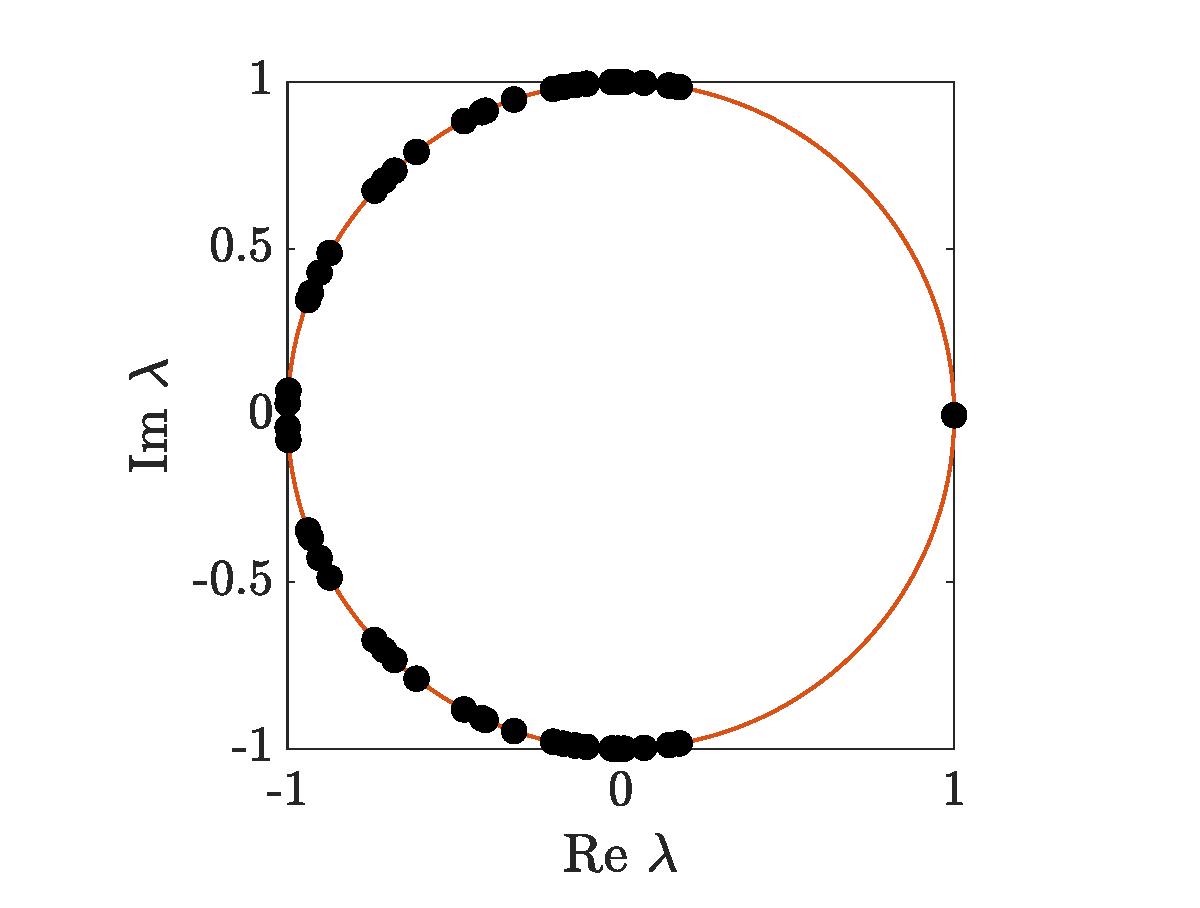
\includegraphics[width=7.5cm]{singlespec.eps} \\ 
	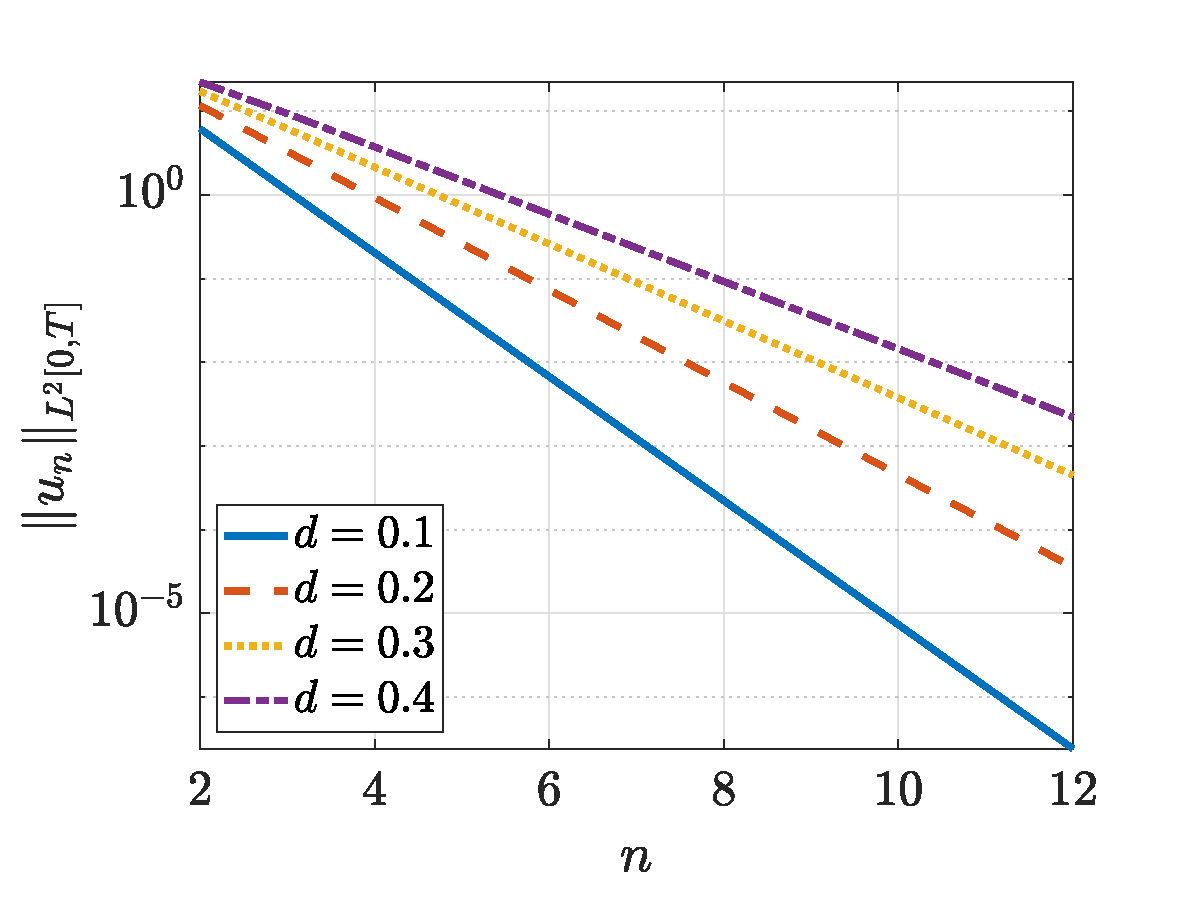
\includegraphics[width=7.5cm]{singledecay.eps} &
	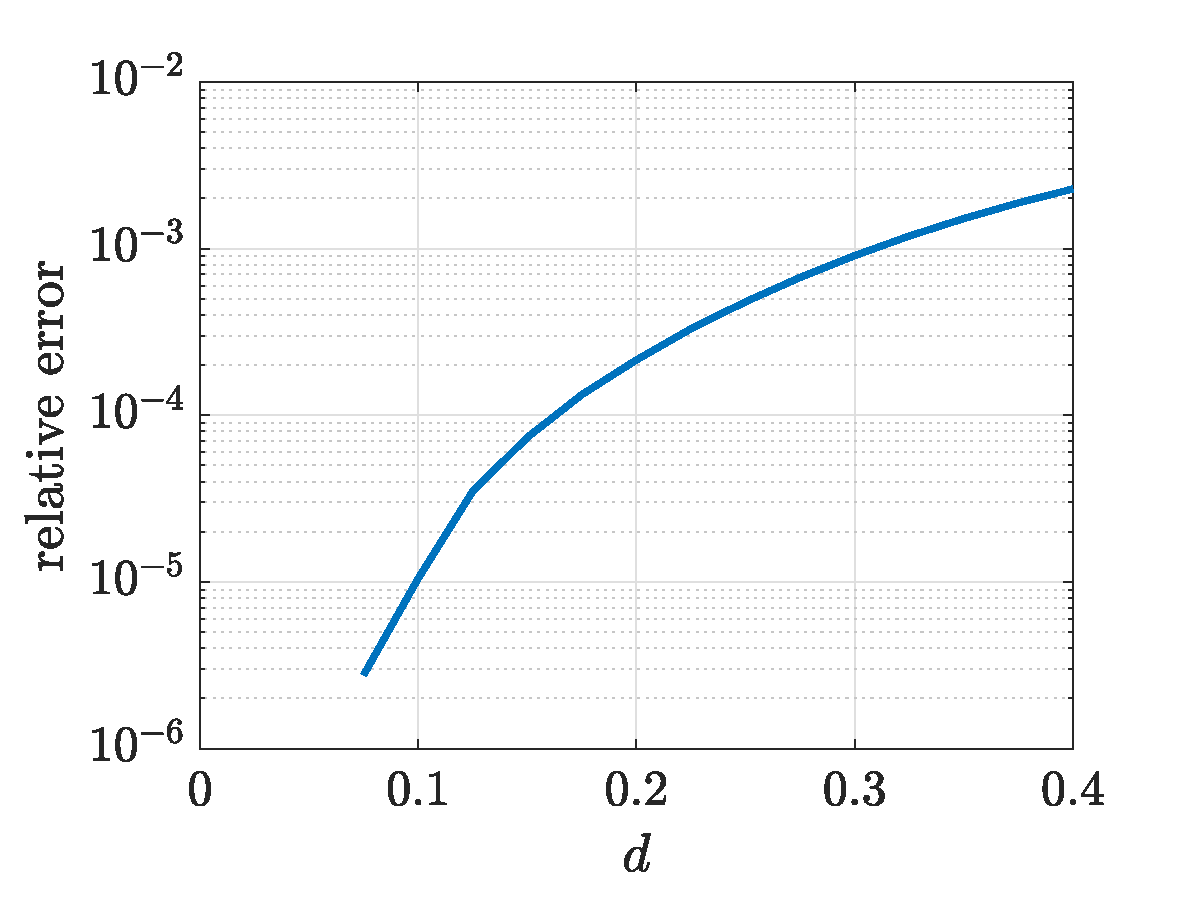
\includegraphics[width=7.5cm]{singledecayerror.eps}
	\end{tabular}
	\end{center}
	\caption{Single}
	\label{fig:single}
\end{figure}

\begin{figure}
	\begin{center}
	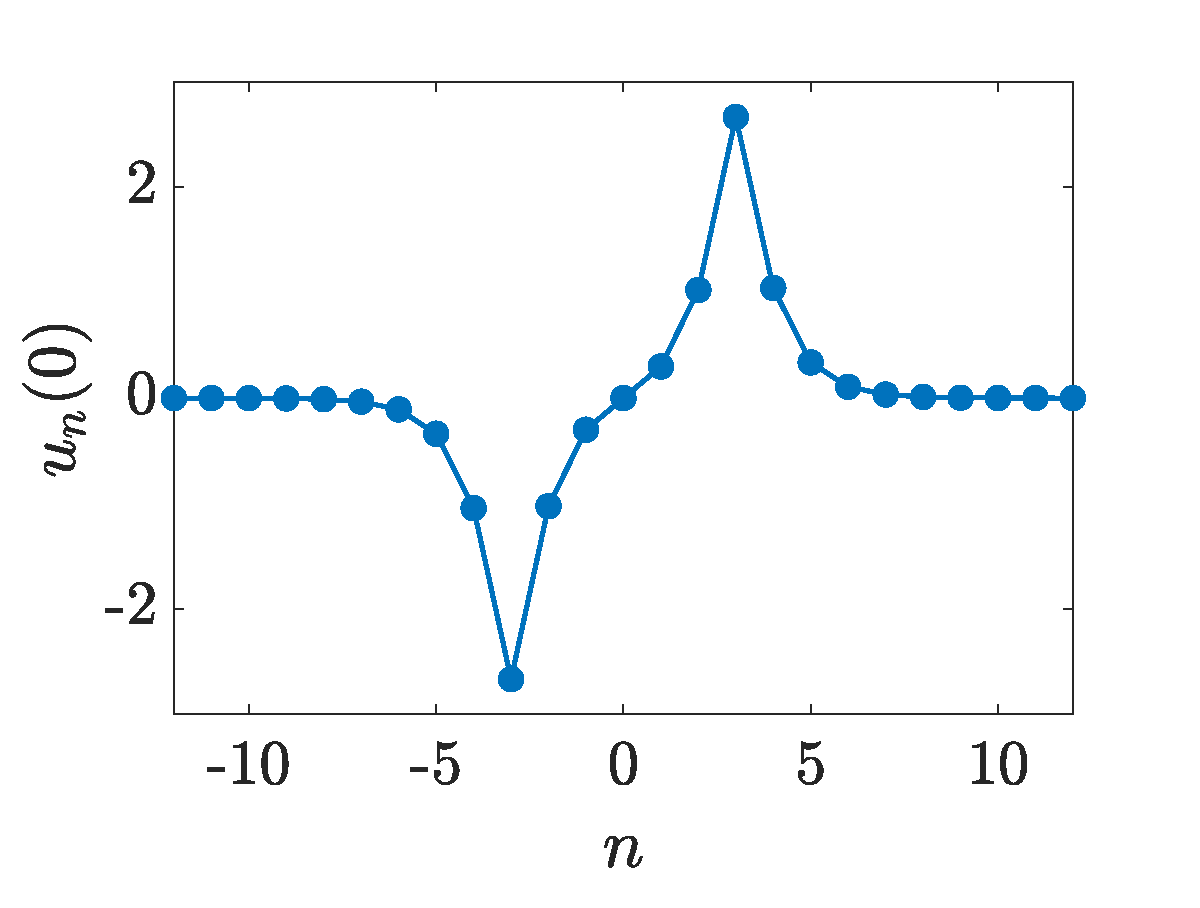
\includegraphics[width=5.5cm]{doubleun0.eps} \hspace{-0.5cm}
	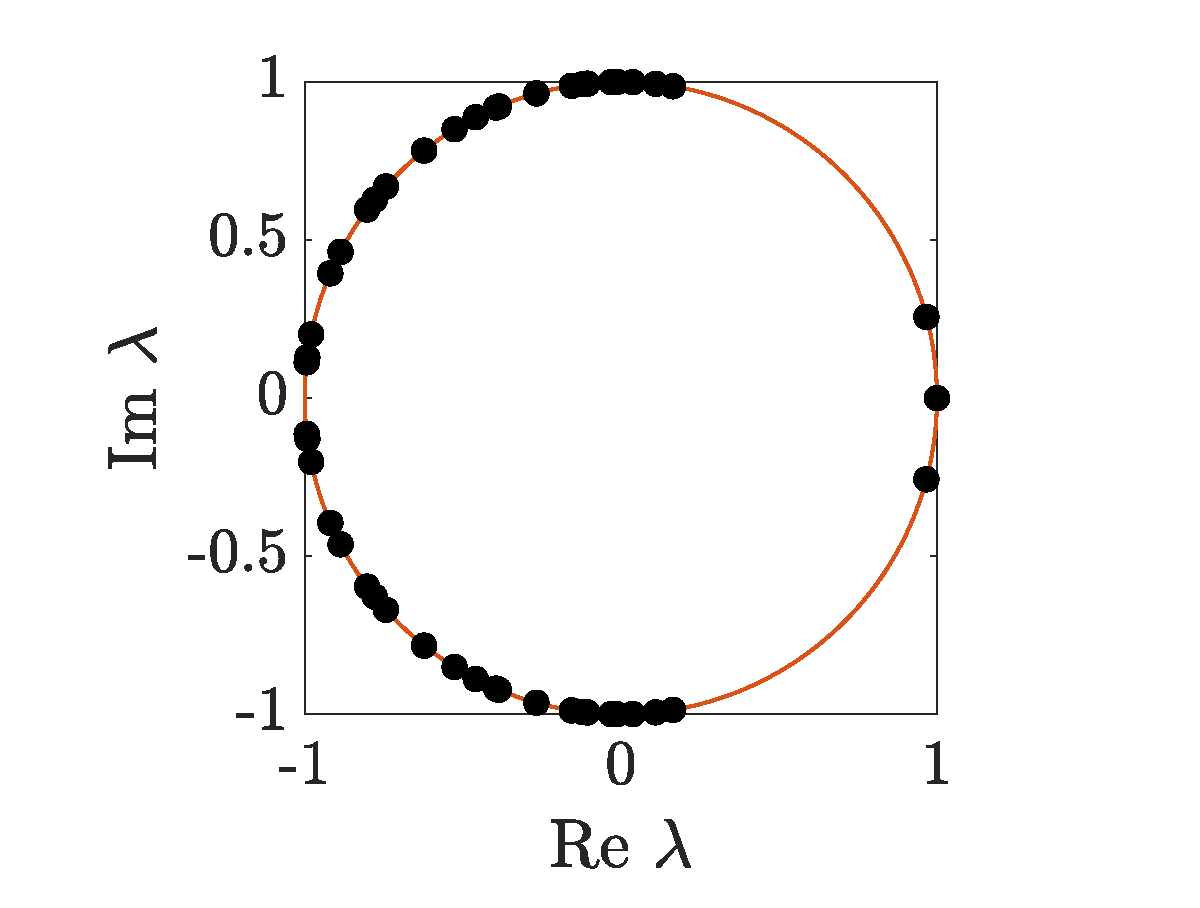
\includegraphics[width=5.5cm]{doublespec.eps} \hspace{-0.5cm}
	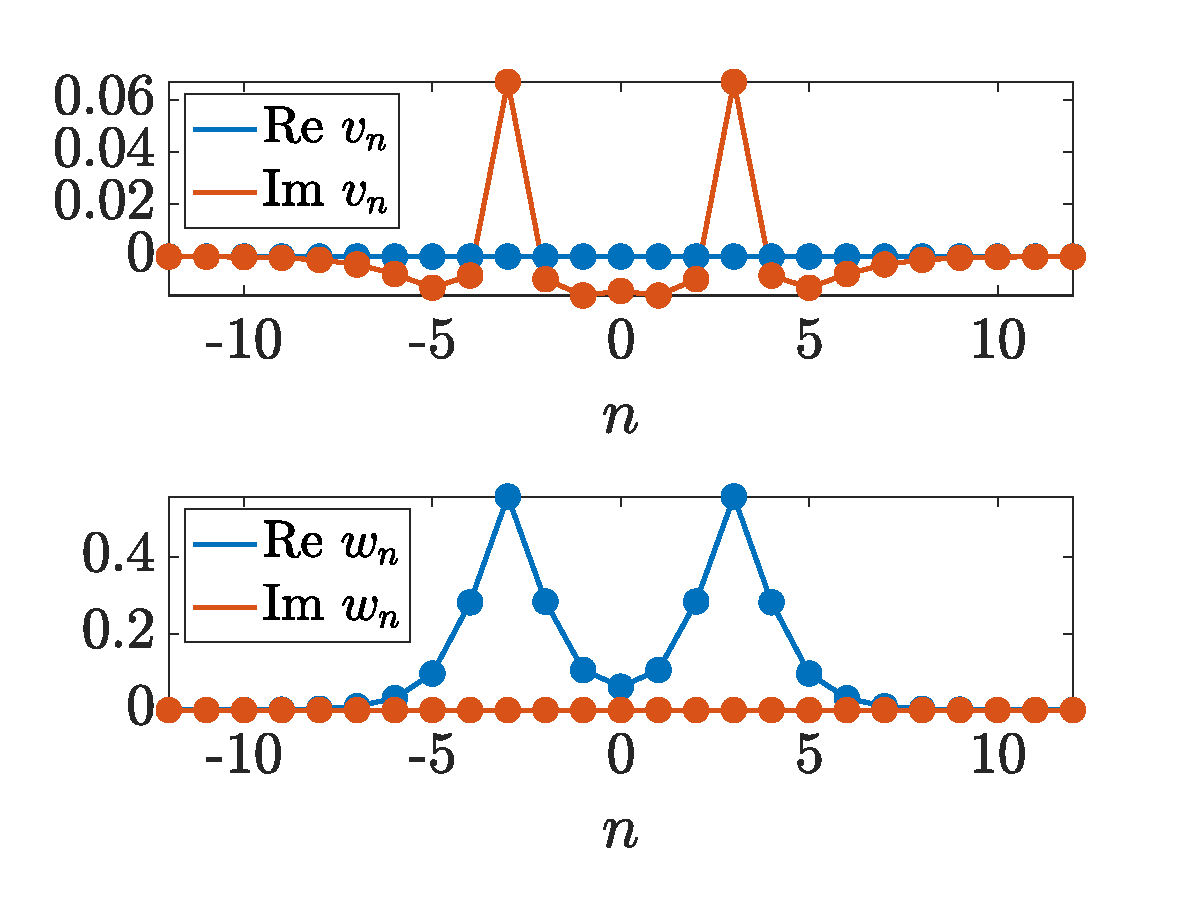
\includegraphics[width=5.5cm]{doubleinteig.eps} 
	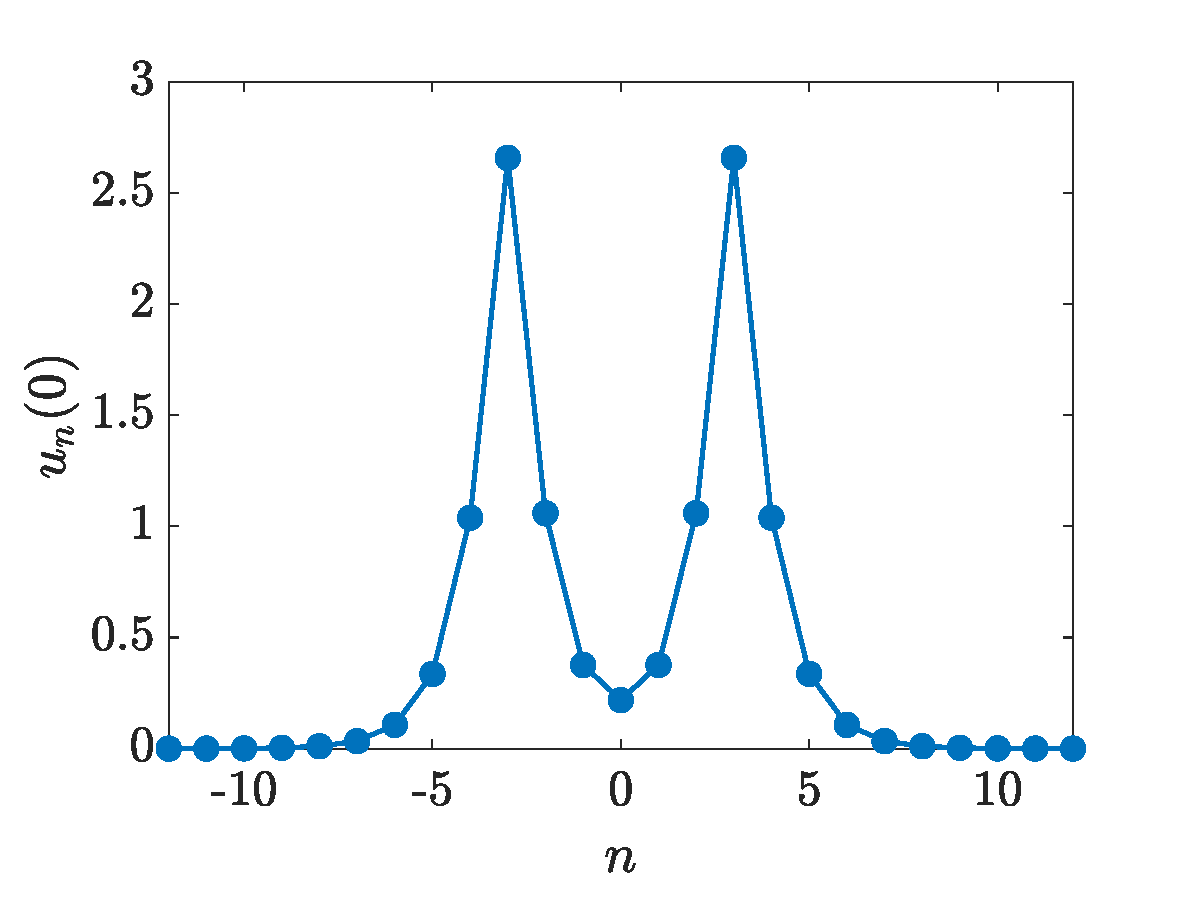
\includegraphics[width=5.5cm]{doubleppun0.eps} \hspace{-0.5cm}
	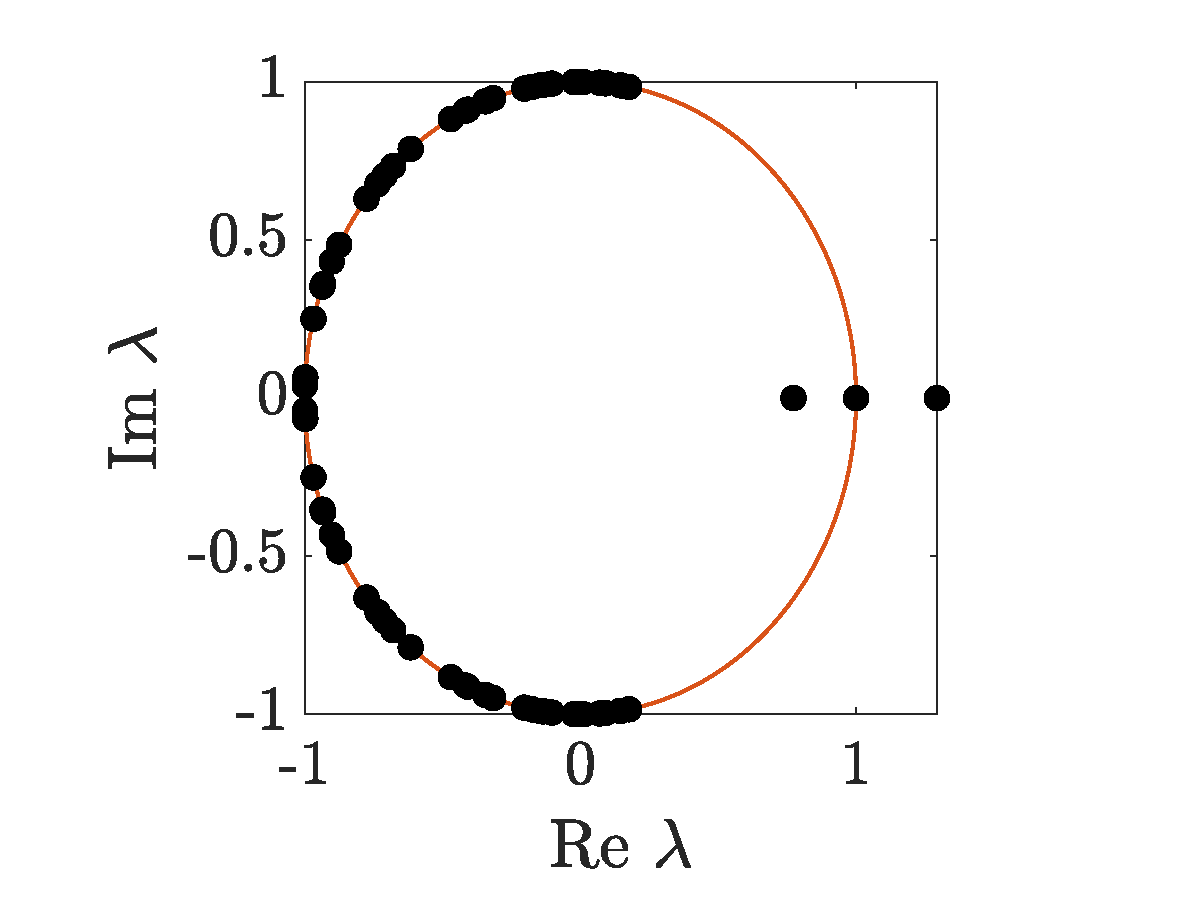
\includegraphics[width=5.5cm]{doubleppspec.eps} \hspace{-0.5cm}
	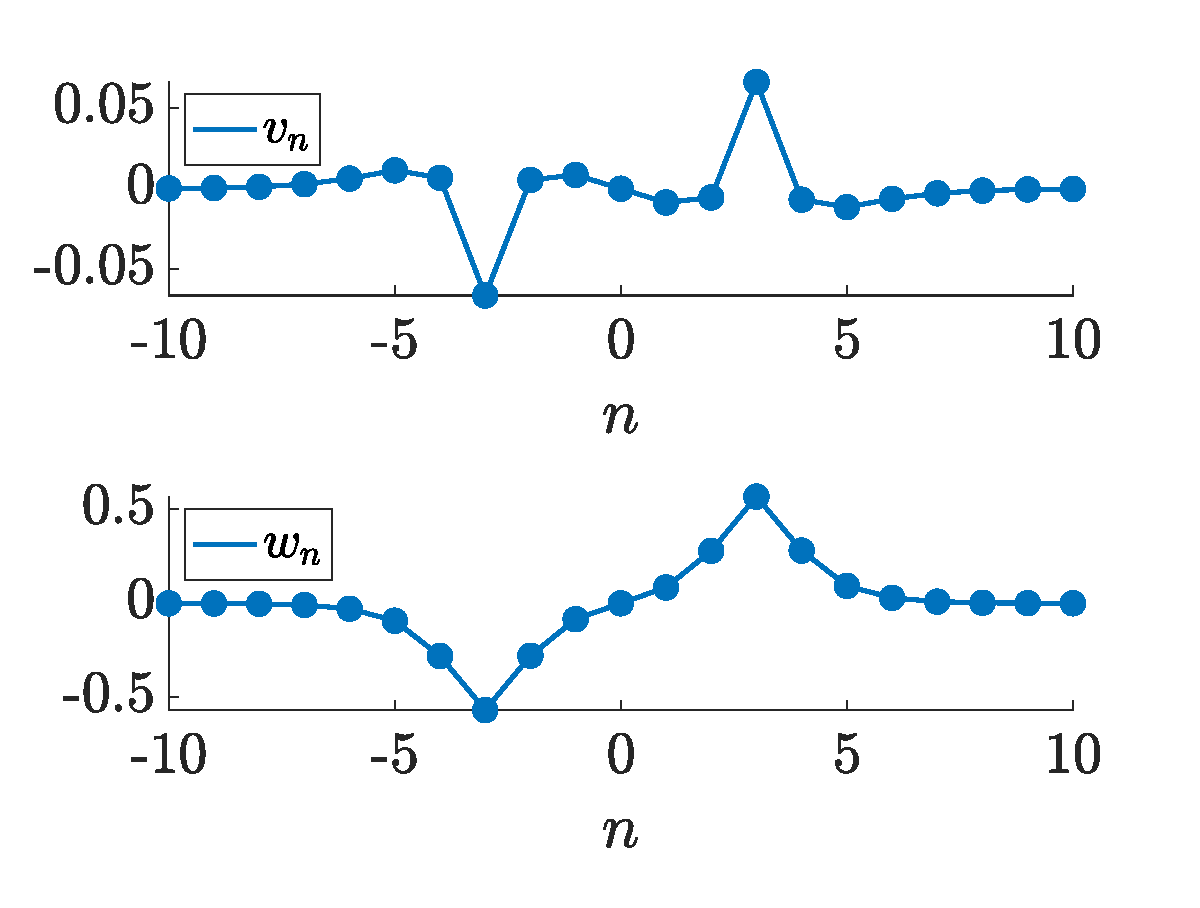
\includegraphics[width=5.5cm]{doubleppinteig.eps} 
	% \end{tabular}
	\end{center}
	\caption{Double}
	\label{fig:double}
\end{figure}

\begin{figure}
	\begin{center}
	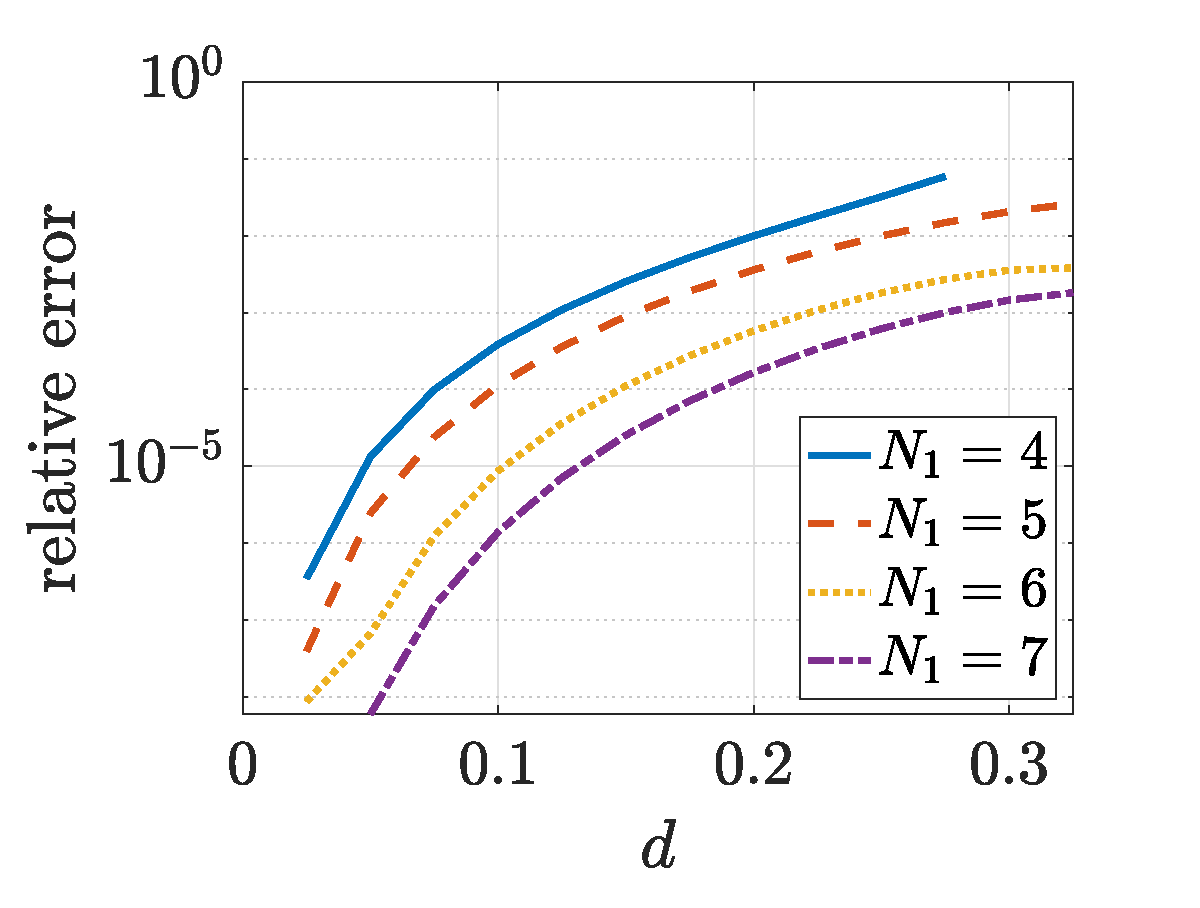
\includegraphics[width=5.5cm]{doubleeigerrord.eps} \hspace{-0.5cm}
	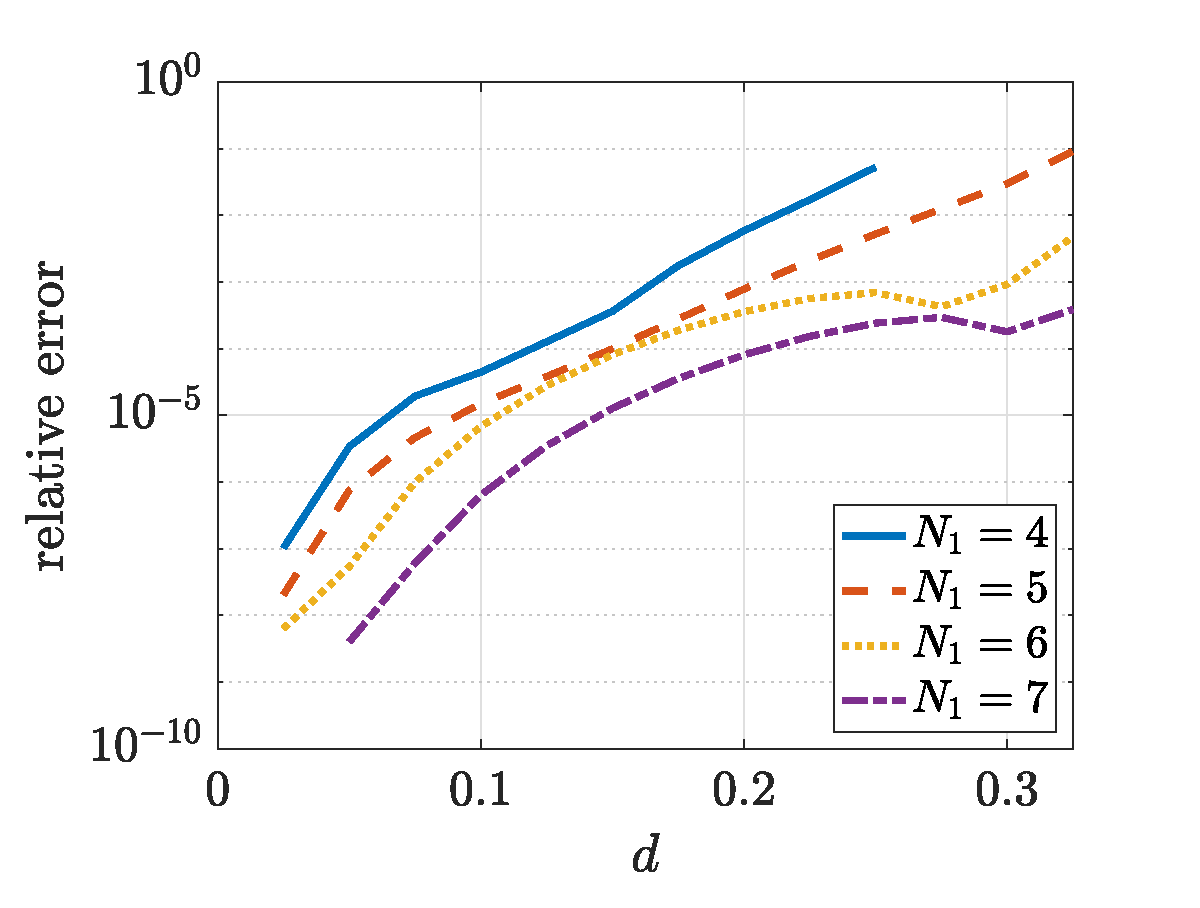
\includegraphics[width=5.5cm]{doubleppeigerrord.eps} \hspace{-0.5cm}
	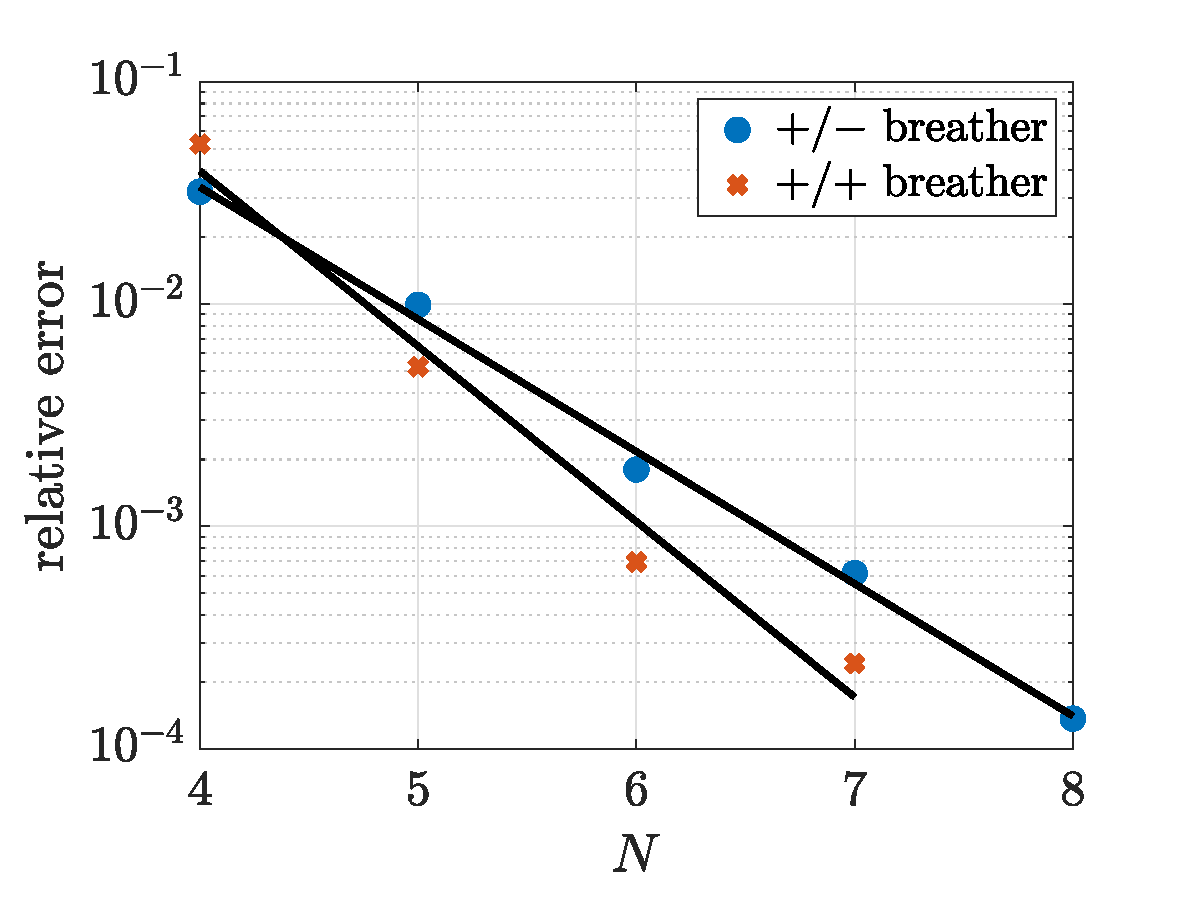
\includegraphics[width=5.5cm]{doubleeigerrorN.eps} 
	% \end{tabular}
	\end{center}
	\caption{Eigenvalue error plots}
	\label{fig:eigerror}
\end{figure}



\paragraph{Acknowledgments}

This material is based upon work supported by the U.S. National Science Foundation under the RTG grant DMS-1840260 (R.P. and A.A.)
and DMS-1809074 (P.G.K.).

\bibliographystyle{amsplain}
\bibliography{DKG.bib}

\end{document}